
\section{Software}
\subsection{Searching in general}
Since a significant part of our project is related to searching, we find it resonable to include a section on how a search engine works in general. The engine consists of two parts: the inverted index and the postings file, and must perform two tasks: indexing and searching.

When performing the indexing task, a loop runs over all the documents in the corpus. For every term encountered in a document, the token\footnote{A token what is left after preprocessing a term. This preprocessing usually includes stemming and removal of special characters.} is added to a dictionary and the document id is appended to the token's postings list. A counter is also kept along with the id to keep track of multiple occurences of the same token in the same document.

The result of this loop is a dictionary of all tokens encountered along with postings lists naming all the documents that contain each token. This dictionary is split into two parts: a postings file containing all the  postings lists written to disk in binary, and an inverted index containing the token, a pointer the token's corrensponding postings list and the number of documents containing the token.

\begin{figure}
    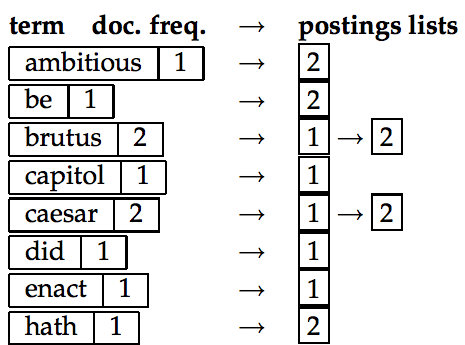
\includegraphics[width=0.5\textwidth]{software/index_postings_lists}
    \caption{A sample index and postings list.}
    \label{fig:index_postings_lists_sw}
\end{figure}

In the searching step one is usually working with a query containing one or more terms. For each token the corrensponding postings list is fetched from disk. Each document is then scored according to a scoring scheme and a list of the documents sorted by the score is returned to the application.\cite{IntroIR}



\subsection{Operating system and environment}
\subsection{Load generator}
The purpose of the load generator is to generate psudo-random queries and send these to the load distributor to simulate load on the cluster. These queries are of varying length and contains a subset of the tokens found in the dictionary. It also includes some tokens not found in the dictionary.

The load generator runs on several threads, where one thread is responsible for receiving answers for the queries, and one or more threads are responsible for generating load for the system. The load generator is implemented in python and ment to be run on a node outside the cluster.

The load generator includes some configurable parameters, most importantly the frequency of the queries being sent and the number of threads sending queries simultaneously.

\subsection{Load distribution}
One of the nodes in the cluster will be in charge of load distribution. This node will receive all the queries and then forward them to the worker nodes. This node has information about the other nodes will spread the workload across the cluster. Since all communication has to go through this node we could end up with the performance of the cluster being limited by the load distributor.

\subsection{Original python version}

\subsection{Optimized C-port}
In practice we experienced serious performance issues with our python code, often showing response times in the hundreds of milliseconds. We therefore decided to rewrite the program using C. This also proved useful to control what exactly is present in memory at every moment, in addition to the extra work of having to control memory allocation.
\subsubsection{Problems}
The first testings of the

